\documentclass[11pt,a4paper]{article}
\usepackage[T1]{fontenc}
\usepackage[utf8]{inputenc}
\usepackage{lmodern}
\usepackage{amsmath,amssymb,amsthm,mathtools}
\usepackage{geometry,graphicx,booktabs,array,longtable,enumitem}
\usepackage{hyperref,xcolor,microtype,fancyhdr}
\geometry{top=24mm,bottom=24mm,left=24mm,right=24mm}
\hypersetup{colorlinks=true,linkcolor=blue!65!black,urlcolor=blue!65!black,citecolor=blue!65!black,pdftitle={FibonacciTopoNet v5.1: Memory, Symmetry and Identifiability},pdfauthor={Research working manuscript; author approval pending}}
\pagestyle{fancy}\fancyhf{}\fancyhead[L]{FibonacciTopoNet v5.1: audited research manuscript}\fancyhead[R]{17 October 2026}\fancyfoot[C]{\thepage}\setlength{\headheight}{14pt}
\theoremstyle{plain}\newtheorem{theorem}{Theorem}[section]\newtheorem{proposition}[theorem]{Proposition}\newtheorem{lemma}[theorem]{Lemma}
\theoremstyle{definition}\newtheorem{definition}[theorem]{Definition}\newtheorem{remark}[theorem]{Remark}\newtheorem{counterexample}[theorem]{Counterexample}
\newcommand{\R}{\mathbb R}\newcommand{\C}{\mathbb C}\newcommand{\Z}{\mathbb Z}\newcommand{\EE}{\mathbb E}\newcommand{\norm}[1]{\left\lVert #1\right\rVert}\newcommand{\tr}{\operatorname{tr}}\newcommand{\rank}{\operatorname{rank}}\newcommand{\diag}{\operatorname{diag}}\newcommand{\softmax}{\operatorname{softmax}}\newcommand{\Span}{\operatorname{span}}\newcommand{\NOTE}{\textsc{Status:}}
\begin{document}
\begin{titlepage}
\centering\vspace*{25mm}
{\large\textsc{Research Monograph / Preprint --- Not Peer Reviewed}\par}
\vspace{14mm}
{\Huge\bfseries FibonacciTopoNet v5.1\\[4mm]
Memory, Symmetry, and Identifiability in a Hybrid Neural--Algorithmic Architecture\par}
\vspace{9mm}
{\large Mathematical Foundations, Audited Implementation, Reproducible Experiments, and Scientific Limits\par}
\vspace{16mm}
{\large Working scientific manuscript --- author approval pending\par}
\vspace{6mm}17 October 2026\par
\vfill
\begin{minipage}{0.87\linewidth}
\textbf{Research status.} A narrowly tested architecture with mathematically auditable components. No claim of frontier-model superiority, peer-reviewed novelty, experimental quantum gravity, general-purpose reasoning, persistent homology, or a physical theory of neural intelligence.
\par\medskip
\textbf{Code and provenance.} \url{https://github.com/4vmp5pkwz4-pixel/HCC/pull/516}; original FibonacciTopoNet v5 and corrected v5.1 retained separately. The META--CAUSAL / $S^3$ physical manuscript is not superseded by this work.
\end{minipage}
\vfill
\end{titlepage}
\begin{abstract}
We develop and critically evaluate FibonacciTopoNet v5.1, a compact sequence-classification prototype combining causal local multiscale attention, a contractive recurrent transform derived from the Fibonacci companion matrix, per-sequence differentiable delta-rule fast weights, an explicitly versioned symbolic key--value store, and an optional projector for a specified harmonic representation of the quotient $S^3/\Z_p$. The corrected version addresses architectural deficiencies of an original v5 prototype: reversal-insensitive classification, nonfunctional memory updates, unsuitable rank-collapse penalties, and an incorrectly identified ``Fibonacci'' recurrence. We prove the obstruction imposed by reversal invariance on balanced anti-symmetric labels; an operator-norm bound $\norm{W}_2<0.93$ for the recurrent linear component; the finite cyclic character-projector identities; a conditional overwrite identity for delta memory; and the behavior of a centered covariance effective-rank proxy. A 2,825-check structural test suite reports no failures. In a narrow paired marker-order benchmark (two seeds, 220 training steps, 512 held-out examples per condition), the original and corrected models achieve 50\% and 100\% at training length 12, respectively; at unseen length 24, the corrected models obtain 99.8047\% and 100\%. These results demonstrate an architectural correction on one synthetic task, not general intelligence, scaling, or superiority over strong baselines. We separate exact symbolic operations from learned memory and mathematical group representations from physical cosmological inference, and state falsifiable requirements for future evaluations.
\end{abstract}
\tableofcontents\clearpage

\section{Scientific scope, contributions, and provenance}
The term \emph{topological network} can denote at least three non-equivalent objects: (i) a learned architecture incorporating discrete or continuous group symmetries, (ii) a network with topological data analysis features such as persistent homology, or (iii) a model operating on a specified geometric manifold, for example the group manifold $SU(2)\cong S^3$. This work implements an explicitly defined example of (i) and a restricted spectral primitive for (iii). It does \emph{not} compute persistent homology, prove a continuum physical limit, or claim that natural-language token embeddings intrinsically live on $S^3$.

The contribution is a carefully scoped synthesis, not a priority claim about independently new components. Local causal attention, recurrent state-space computation, delta-rule fast weights, group averaging, and exact key--value stores each have substantial precedents. Relevant benchmarks and prior methods include group-equivariant networks \cite{cohen2016,bronstein2021}, fast-weight programmers \cite{schlag2021}, structured state-space models \cite{dao2024,gu2022}, and long-term neural memory \cite{behrouz2025}. The scientific value of this edition rests in explicit assumptions, testable equations, a failure-mode audit, and reproducible observations.

\subsection{Provenance and scope of the source models}
Version v3 implemented a causal memory architecture; v4 added differentiable and algorithmic key--value memory and carefully limited synthetic tests; the user-supplied original v5 combined several modules but showed errors in symmetry, memory semantics, and regularization. The corrected v5.1 is retained as a separately versioned snapshot. The exact original is archived byte-for-byte in the research release. The distinct physical monograph META--CAUSAL / $S^3$ v244 addresses conditional cosmological spectral constructions; none of those physical claims are established by this neural network.

We use three epistemic labels throughout: \textbf{mathematical} (deduction under explicit definitions), \textbf{numerical} (a finite test or measurement), and \textbf{hypothetical} (an untested possibility). Numerical test passage does not imply formal proof, and an operational analogy is not a physical law.

\section{Architecture and computational model}
Let $x_0,\ldots,x_{T-1}$ be tokens in a finite vocabulary; $E(x_t)\in\R^d$ is the learned embedding, augmented with sinusoidal positions $p_t$. Write
\begin{equation}
 z_t^{(0)}=E(x_t)+p_t,\qquad
 p_{t,2j}=\sin(t\omega_j),\quad p_{t,2j+1}=\cos(t\omega_j),\quad \omega_j=10000^{-2j/d}.
\end{equation}
The encoder consists of causal local attention and pointwise feed-forward sublayers with residual normalization. The prototype uses window lengths derived from $[1,2,3,5]$; Fibonacci numbers are an optional sampling policy rather than a proven optimal scale schedule.

\subsection{Causal multiscale attention}
For each head, query $q_t$, key $k_s$ and value $v_s$ are obtained by linear projections. At scale $w$ define the past-only index set $\mathcal J_w(t)=\{s: \max(0,t-w)\le s\le t\}$. Then
\begin{equation}\label{eq:local}
 a_t^{(w)}=\sum_{s\in\mathcal J_w(t)}\frac{\exp(q_t^\top k_s/\sqrt{d_h})}{\sum_{u\in\mathcal J_w(t)}\exp(q_t^\top k_u/\sqrt{d_h})}v_s,
 \qquad a_t=\sum_{w\in\mathcal W}\pi_w a_t^{(w)},\quad \pi=\softmax(\alpha).
\end{equation}
The implementation's \verb|CausalLocalAttention| constructs only the queried local key/value windows, rather than the dense $T\times T$ attention-score array. The attention arithmetic is $O(BHd_hT\sum_w(w+1))$ up to projections and implementation overhead. Importantly, the \emph{complete model} also executes $O(Td^2)$ recurrence and fast-weight updates, so it is incorrect to assign this local-attention complexity to the whole model.

\begin{proposition}[Causality of the local attention layer]\label{prop:causality}
Assume that all key, value and query projections act pointwise on the current token features; the normalization statistics are per token; all attention windows lie in $\{0,\ldots,t\}$; and no other network path accesses positions later than $t$. Then the layer output at time $t$ is a function solely of inputs at positions $\le t$.
\end{proposition}
\begin{proof}
Every term in \eqref{eq:local} involves $q_t$ and $k_s,v_s$ with $s\le t$; the scale mixing weights are global trainable constants independent of the input sequence. Pointwise residual and feed-forward transformations preserve the dependency property. Composition of these causal maps is causal by induction over depth.
\end{proof}
\begin{remark}
This proposition is about \emph{sequence prefix outputs}. The classifier consumes the final recurrent state and thus naturally uses the entire available input sequence. It does not assert token-by-token autoregressive generation or streaming without recomputation.
\end{remark}

\subsection{The Fibonacci companion transform and bounded recurrence}
Define the golden ratio and its normalized companion matrix by
\begin{equation}\label{eq:fib}
 \varphi=\frac{1+\sqrt5}{2},\qquad
 C_\varphi=\frac1\varphi\begin{pmatrix}1&1\\1&0\end{pmatrix}.
\end{equation}
For even $d$, let $B=\operatorname{diag}(C_\varphi,\ldots,C_\varphi)$. The actual trainable recurrent matrix is
\begin{equation}\label{eq:W}
 W=0.85 B+0.08\,\frac{R}{1+\norm{R}_2},
\end{equation}
where $R\in\R^{d\times d}$ is learned. The recurrent update is
\begin{equation}\label{eq:rec}
 g_t=\sigma(Gz_t+b_g),\quad c_t=\tanh(W h_{t-1}+Uz_t+b_c),\quad h_t=g_t\odot h_{t-1}+(1-g_t)\odot c_t.
\end{equation}
A padding mask holds the previous state at invalid positions. The learned matrix $W$ is a contractive linear component, but the gated input-dependent update is nonlinear and is not thereby proved globally contractive in the entire input--state space.

\begin{theorem}[Norm bound for the normalized Fibonacci recurrent component]\label{th:op}
For the matrix $W$ in \eqref{eq:W}, with $d$ even and finite $\norm{R}_2$, one has $\norm{W}_2<0.93$ for every learned $R$.
\end{theorem}
\begin{proof}
The unscaled companion matrix $\left(\begin{smallmatrix}1&1\\1&0\end{smallmatrix}\right)$ is symmetric, with eigenvalues $\varphi$ and $-\varphi^{-1}$. Hence $C_\varphi$ has eigenvalues $1,-\varphi^{-2}$, and its spectral norm is exactly 1. A block-diagonal repetition also has norm 1. By the triangle inequality and submultiplicativity,
$\norm{W}_2\le0.85+0.08\norm{R}_2/(1+\norm{R}_2)<0.93$.
\end{proof}

\begin{proposition}[Bounded hidden coordinates]\label{prop:box}
If $h_0\in[-1,1]^d$, the update \eqref{eq:rec} with sigmoid $g_t\in(0,1)^d$ and tanh candidate $c_t\in(-1,1)^d$ satisfies $h_t\in[-1,1]^d$ for all $t$.
\end{proposition}
\begin{proof}
Each coordinate of $h_t$ is a convex combination of two numbers in $[-1,1]$. Induction applies. Masked steps leave $h_{t-1}$ unchanged.
\end{proof}
Theorem \ref{th:op} and Proposition \ref{prop:box} are distinct: a bounded trajectory does not imply bounded gradient propagation, nonexpansive input--output behavior, robust optimization, or long-context generalization.

\subsection{Per-sequence differentiable fast weights}
The functional fast-weight state is $M_t\in\R^{d\times d}$ for each individual sequence, initialized at zero. Given the normalized key $\hat k_t=k_t/\norm{k_t}$, candidate value $v_t$, and update gate $\beta_t\in(0,1)$, the update is
\begin{equation}\label{eq:delta}
 M_t=M_{t-1}+\beta_t\big(v_t-M_{t-1}\hat k_t\big)\hat k_t^\top,
 \qquad r_T=M_T\frac{q_T}{\norm{q_T}}.
\end{equation}
Normalized keys are defined numerically with an epsilon safeguard. This construction performs differentiable writes into an explicit, per-forward state; it does not mutate learned parameter tensors with \verb|.data|, and it does not preserve learned facts across independent forward calls. Connections to fast-weight programming and delta rules are established in \cite{schlag2021}.

\begin{proposition}[Conditional delta overwrite]\label{prop:delta}
For $\norm{\hat k}=1$ and $M'=M+\beta(v-M\hat k)\hat k^\top$,
\begin{equation}
 M'\hat k=(1-\beta)M\hat k+\beta v.
\end{equation}
Consequently, exact overwrite $M'\hat k=v$ holds for $\beta=1$, while a gate $0<\beta<1$ only interpolates. Moreover, any $u\perp\hat k$ has $M'u=Mu$.
\end{proposition}
\begin{proof}
Right-multiply the update by $\hat k$, using $\hat k^\top\hat k=1$. For $u\perp\hat k$, the outer-product correction annihilates $u$.
\end{proof}
\begin{counterexample}[Nonorthogonal key interference]\label{ce:cross}
Take two unit keys $k_1,k_2$ with $k_1^\top k_2\ne0$. An update targeting $k_2$ changes the first readout by
$M'k_1-Mk_1=\beta(v-Mk_2)(k_2^\top k_1)$. Thus a generic finite fast-weight memory does not provide unconditional exact last-write-wins semantics across arbitrary learned keys.
\end{counterexample}

\subsection{The distinct, exact symbolic store}
An \verb|OrderedDict| store maintains pairs $k\mapsto(v,\nu)$ where $\nu$ is a monotonically increasing write version. Deletion, capacity errors and typed links are explicitly represented. Link following distinguishes a reference \verb|MemoryLink("A")| from the literal text \verb|"A"| and terminates with explicit \texttt{known}, \texttt{unknown}, \texttt{cycle}, or \texttt{budget} status. The exact store is a \emph{deterministic algorithmic oracle}, not a learned generative memory, and is not implicitly called by the neural classifier.

\section{Symmetry, identifiability and the cost of invariance}
Symmetries are valuable only if they preserve the target. The representation-theoretic principle behind group-equivariant deep learning is well documented \cite{cohen2016,bronstein2021}. The following elementary theorem supplies an audit standard for \emph{destructive} invariance in classification.

\begin{definition}
For a map $r:\mathcal X\to\mathcal X$ satisfying $r^2=\mathrm{id}$, a classifier $f$ is reversal-invariant if $f(rx)=f(x)$ for every $x$.
\end{definition}
\begin{theorem}[Balanced orbit-pair obstruction]\label{th:reverse}
Let a finite held-out set be the disjoint union of pairs $\{x_i,rx_i\}$, and suppose the target labels satisfy $y(rx_i)=1-y(x_i)$ for each pair. Every deterministic classifier satisfying $f(rx)=f(x)$ on the set has accuracy at most $1/2$.
\end{theorem}
\begin{proof}
Both members of a pair receive the same predicted class but have different binary target classes. At most one of the two predictions is correct. Summing over the pairs yields at most one correct prediction out of each pair of two.
\end{proof}
The original v5 network had symmetric attention neighborhoods, no absolute or relative position feature, and a symmetric token-averaging readout. Subject to symmetric boundary and padding conventions, it is reversal invariant. Its measured maximum logit difference after reversal, approximately $2.98\times10^{-8}$, is compatible with floating-point error rather than meaningful order sensitivity. The corrected architecture replaces this structural loss by causal windows, sinusoidal positions, and an order-sensitive final recurrence. The theorem guarantees the baseline's \emph{ceiling} on the mirrored task; it does not guarantee that a corrected model will train successfully.

\begin{theorem}[Finite-group orbit projection]\label{th:group}
Let $G$ be a finite group, $U:G\to\mathcal U(H)$ a unitary representation on a finite-dimensional complex Hilbert space, and $P=|G|^{-1}\sum_{g\in G}U(g)$. Then $P$ is the orthogonal projector onto $H^G=\{x:U(g)x=x\ \forall g\in G\}$.
\end{theorem}
\begin{proof}
Unitary group averaging is self-adjoint since $g\mapsto g^{-1}$ is a bijection. Moreover
$P^2=|G|^{-2}\sum_{g,h}U(gh)=|G|^{-1}\sum_k U(k)=P$; each $U(h)P=P$. Conversely $Pv=v$ for every invariant vector $v$. Thus the range of $P$ is exactly $H^G$.
\end{proof}
\begin{remark}
An invariant readout collapses all vectors in the same group orbit; it cannot distinguish orbit-dependent labels. Equivariant intermediate representations can preserve more information than an immediately invariant projection. The existence of a mathematically natural symmetry is not evidence that a given language task respects it.
\end{remark}

\section{Exact cyclic harmonic projector on \texorpdfstring{$S^3$}{S3}}
\subsection{Representation convention}
Use $S^3\cong SU(2)$ with a specified cyclic left action $\Z_p\le SU(2)_L$. Degree-$n$ scalar harmonics live in the $(j,j)$ representation of $SU(2)_L\times SU(2)_R$, where $j=n/2$ and the dimension is $(n+1)^2$. Index the left weights by
\begin{equation}
 w=-n,-n+2,\ldots,n,
\end{equation}
with $(n+1)$ copies each for right weights. This convention must be held fixed when comparing coordinates, group actions, or observables; a different embedding $L(p,q)$ requires a different congruence formula.

For character $a\in\{0,\ldots,p-1\}$ define
\begin{equation}\label{eq:cyc}
 P_{n,p,a}=\frac1p\sum_{k=0}^{p-1}\exp\!\left(\frac{2\pi i k(W_n-aI)}p\right),
\end{equation}
where $W_n$ is the diagonal matrix of left weights (each repeated $n+1$ times). This operator is \emph{defined only} on the specified degree-$n$ harmonic coefficient space, not on arbitrary token embeddings.

\begin{theorem}[Cyclic character selection]\label{th:cyc}
Under the conventions above, the entries of the character projector satisfy
\begin{equation*}(P_{n,p,a})_{ww\prime}=\delta_{ww\prime}\,\mathbf{1}_{w\equiv a\;(\mathrm{mod}\,p)}.\end{equation*}
In particular,
\begin{equation}
 P_{n,p,a}^*=P_{n,p,a},\quad P_{n,p,a}^2=P_{n,p,a},\quad P_{n,p,a}P_{n,p,b}=0\ \ (a\ne b),\quad
 \sum_{a=0}^{p-1}P_{n,p,a}=I.
\end{equation}
Its rank is
\begin{equation}\label{eq:rank}
 \rank P_{n,p,a}=(n+1)\sum_{r=0}^{n}\mathbf1_{-n+2r\equiv a\;(\mathrm{mod}\,p)}.
\end{equation}
\end{theorem}
\begin{proof}
The diagonal entry of \eqref{eq:cyc} at weight $w$ is the finite geometric sum
$p^{-1}\sum_{k=0}^{p-1}e^{2\pi i k(w-a)/p}$, equal to one if $p\mid(w-a)$ and zero otherwise. All identities and the rank formula follow from the diagonal selection masks.
\end{proof}
\begin{counterexample}[Arbitrary embeddings are not harmonic coefficients]
A vector $z\in\R^{(n+1)^2}$ produced by a text embedding has no canonical left-$SU(2)$ weight labeling. Applying a numerical mask with the correct shape does not automatically endow $z$ with a $\Z_p$ action or preserve physical gauge symmetries. Without an equivariant feature construction or a stated data-to-harmonics map, identifying this mask as physical topological inference is unjustified.
\end{counterexample}

Theorem \ref{th:cyc} is a standard finite character-orthogonality specialization. Its inclusion makes the computational contract explicit and testable, not a discovery of a new $S^3$ spectral law. The scalar quotient mode count is independent of any hypothesized new gravity dynamics.

\section{Spectral diversity proxy versus genuine topology}
For centered feature samples $z_i=x_i-\bar x\in\R^d$, define the empirical covariance
\begin{equation}
 C=\frac1{m-1}\sum_{i=1}^m z_iz_i^\top,\qquad C\succeq0.
\end{equation}
When $\tr C>0$, define $\kappa(C)=\tr(C^2)/(\tr C)^2$. The actual regularizer is proportional to $\max(0,\kappa(C)-1/r_{\max})$ where $r_{\max}=\min(d,m-1)$. A separate finite value handles zero variance.
\begin{proposition}[Centered spectral participation bound]\label{th:rank}
If $C\succeq0$ has nonzero eigenvalues $\lambda_1,\dots,\lambda_r>0$, then
\begin{equation}
 \frac1r\le\kappa(C)=\frac{\sum_{i=1}^r\lambda_i^2}{(\sum_{i=1}^r\lambda_i)^2}\le1.
\end{equation}
The lower bound holds at equal nonzero eigenvalues; the upper bound is achieved for rank one.
\end{proposition}
\begin{proof}
Cauchy--Schwarz yields $(\sum_i\lambda_i)^2\le r\sum_i\lambda_i^2$, implying $\kappa\ge1/r$. Also $(\sum_i\lambda_i)^2=\sum_i\lambda_i^2+2\sum_{i<j}\lambda_i\lambda_j\ge\sum_i\lambda_i^2$, implying $\kappa\le1$.
\end{proof}
The penalty is translation-invariant due to centering and detects rank-one concentration relative to a well-spread spectrum. It is \emph{not} the spectral gap of a Hodge Laplacian, a persistent-homology barcode, or a proof of stable semantic manifolds. Genuine topological penalties would require a specified complex, boundary operators and filtration (or a defined geometric manifold and Laplacian).

\section{Controlled experiments and audit results}
\subsection{Experiment design and observations}
Each benchmark instance asks whether marker $A$ appears before marker $B$, with reversed sequence paired with an opposite target. Training length $T=12$, out-of-distribution test length $T=24$, two random seeds, 220 optimization steps, and 512 held-out examples for each length/seed. The results are copied from the committed \texttt{ORDER\_BENCHMARK.json}; the current monograph does not claim a newly trained benchmark with further hyperparameter tuning. The benchmark fits a narrow, binary rule with a deliberately symmetry-breaking label function.
\begin{table}[ht]
\centering
\caption{Two-seed marker-order benchmark from the audited research archive. Time measured for the reported CPU training runs.}
\label{tab:benchmark}
\begin{tabular}{@{}llrrr@{}}\toprule
Model & Seed & Parameters & Acc. $T=12$ & Acc. $T=24$\\\midrule
Original v5 & 17 & 10,039 & 50.00\% & 50.00\%\\
Original v5 & 29 & 10,039 & 50.00\% & 50.00\%\\
Corrected v5.1 & 17 & 8,913 & 100.00\% & 99.8047\%\\
Corrected v5.1 & 29 & 8,913 & 100.00\% & 100.00\%\\\bottomrule
\end{tabular}
\end{table}
\begin{figure}[ht]\centering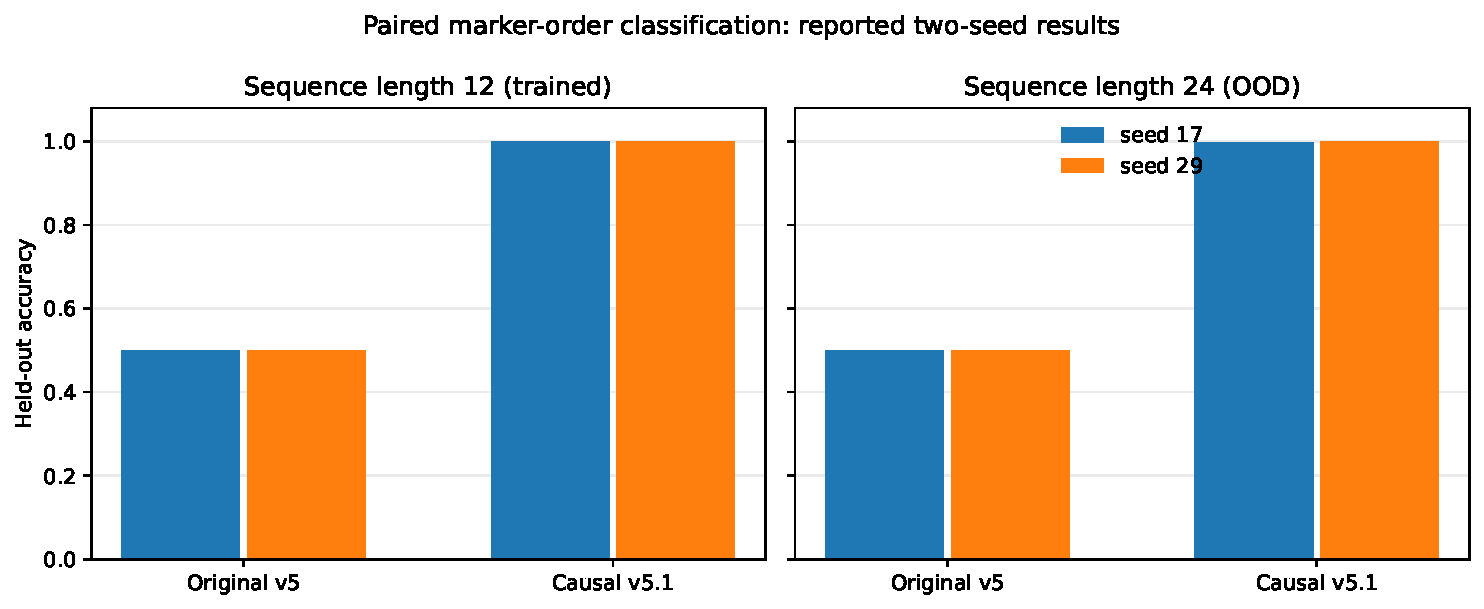
\includegraphics[width=.94\linewidth]{figures/marker_order.pdf}\caption{Descriptive results for the source-controlled two-seed paired marker-order benchmark. $T=24$ is a modest OOD length change, not general long-context success.}\label{fig:benchmark}\end{figure}
The 69,083-parameter number cited for the user's original v5 refers to a \emph{different smoke-test configuration}, which memorized a tiny randomly labeled \emph{training} batch. It must not be interchanged with the 10,039-parameter baseline used here. Corrected v5.1 required approximately 4.7--5.13 CPU seconds for 220 steps against 2.49--2.61 seconds for the smaller original-v5 benchmark setting. A lower parameter count is therefore not evidence of lower wall-clock cost.

A 50\% score for the original model is expected from Theorem \ref{th:reverse}; an improvement of the corrected model is consistent with restoring order information. The benchmark is not capable of separating the benefits of positional features, causality, recurrence, fast weights, and window ratios because no complete one-factor-at-a-time ablation is provided. It also does not compare a matched Transformer, GRU, Mamba-2 or Titans with equivalent training compute.

\subsection{Verification matrix}
The separate \texttt{verify\_v5\_1.py} output reports 2,825 passed checks and zero failures. The main categories are causal local/dense equivalence, no-future dependence, padding isolation, recurrent operator norm, hidden-state boundedness, centered covariance behavior, memory updates and gradient flow, and quotient projector properties. Most checks (1,170+1,170) sweep cyclic projection and its finite group-average form across degrees, orders and characters. Thus the number 2,825 does \emph{not} mean 2,825 independent machine-checked theorems or 2,825 independent neural experiments.
\begin{table}[ht]
\centering\caption{Selected entries from the archived test report.}\begin{tabular}{@{}lrr@{}}\toprule
Category & Checks & Failures\\\midrule
Idempotence of cyclic projectors & 1,170 & 0\\
Agreement with finite group average & 1,170 & 0\\
Character-sector resolution & 156 & 0\\
$S^3$ projector rank & 156 & 0\\
Contractive recurrent operator bound & 45 & 0\\
Bounded recurrence trajectories & 45 & 0\\
Causal future independence & 14 & 0\\
Padding independence & 14 & 0\\
Remaining audit categories & 55 & 0\\\midrule
\textbf{Total} & \textbf{2,825} & \textbf{0}\\\bottomrule\end{tabular}\end{table}
\begin{figure}[ht]\centering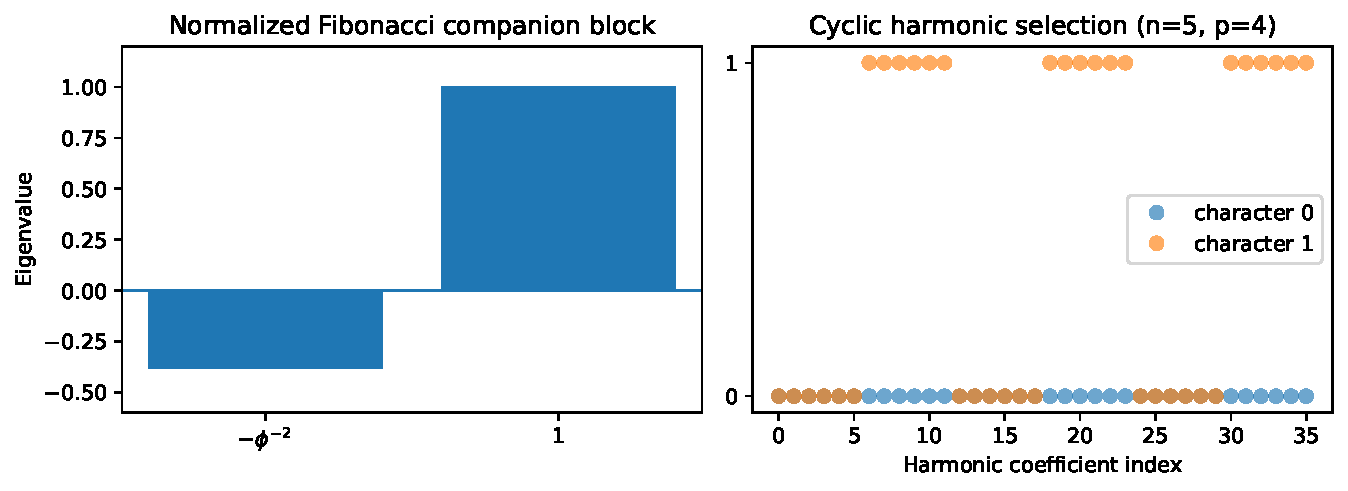
\includegraphics[width=.88\linewidth]{figures/math_components.pdf}\caption{Left: spectrum of the normalized companion block, whose spectral norm equals one. Right: character selection in the specified left-weight harmonic basis. Neither graph asserts a physical neural manifold.}\end{figure}

\subsection{Limitations of statistical interpretation}
Only two seeds are available. The paired reversed examples are dependent, so naive independent-binomial confidence intervals using 512 samples would overstate the available information. No uncertainty band over initialization, optimizer noise, data distribution, or hyperparameter selection is claimed. There is no credible frontier-model comparison based on this dataset alone. Further, a classifier trained on one handcrafted binary relation cannot by itself demonstrate language modeling, logical reasoning, stable continual learning, or world-model construction.

\section{The exact boundary between geometry, physics and computation}
The mathematical bridge from the physical META--CAUSAL/$S^3$ project to the neural prototype is an \emph{operator motif}: finite-group averaging identifies invariant subspaces; representation labels select sectors; covariance operators measure second-order properties; and an explicit observer/readout map can discard identifiable information. The bridge is structurally meaningful but insufficient to transfer dynamical equations or empirical CMB claims. In particular, the following statements are excluded from the present results:
\begin{enumerate}[leftmargin=*,itemsep=1pt]
\item A language token has a canonical location on $S^3$ or a physically meaningful $SU(2)$ action.
\item The quotient harmonic projector implements a tensor-spin $2$ Einstein--Boltzmann transport operator.
\item A general neural covariance regularizer computes Hodge Laplacians or topological Betti numbers.
\item The Fibonacci eigenvalue $\varphi$ is a universal optimum for neural memory dynamics.
\item Symbolic exact memory is a learned end-to-end model of factual reliability.
\item Structural tests establish quantum gravity, cosmological topology, or a new universal law of intelligence.
\end{enumerate}
This separation is essential for future independent research: the right equivalence notion is determined by the application, and both quotienting and pooling can irreversibly erase label-relevant information.

\section{Reproducibility and independent verification protocol}
\subsection{Source-controlled evidence}
The scientific artifact is the release comprising the user's unmodified original v5 file, corrected v5.1 module, audit tests, paired benchmark, four saved checkpoints, dependency specification, and SHA256 checksums. These are preserved in the project branch and draft pull request at \url{https://github.com/4vmp5pkwz4-pixel/HCC/pull/516}. The manuscript belongs in an additional independent documentation revision; approval is required before a merge into the HCC production branch.

\subsection{Exact reproduction steps}
\begin{enumerate}[leftmargin=*]
\item Obtain the v5.1 research directory and verify \verb|sha256sum -c SHA256SUMS.txt| using the checksums recorded with that snapshot (paths are relative to the appropriate source root).
\item Create a clean Python virtual environment, install the recorded PyTorch dependency, record Python, operating system, CPU/GPU and PyTorch versions.
\item Run \verb|python verify_v5_1.py| and archive its full stdout and exit status.
\item Run \verb|python benchmark_order.py| with the documented seeds and configurations; compare all JSON scalars rather than selectively reporting best runs.
\item Load demonstration checkpoints only from trusted sources, setting \texttt{weights\_only=True} in \texttt{torch.load}. Use the exact benchmark constructor parameters.
\item Repeat training under additional initialization seeds and compare to parameter- and compute-matched no-Fibonacci, Transformer, GRU and state-space controls.
\item Perform at least one independently implemented quotient-projector calculation without reusing the same indexing routine as the model, and test orientation/basis conventions explicitly.
\end{enumerate}
The original regression record, not the present paper, is the source of the reported 2,825 tests and accuracy measurements. The manuscript can be compiled independently by two runs of \verb|pdflatex|.

\section{Research roadmap and falsifiable gates}
The next research milestone is not another count of unvalidated ``fundamental laws''. It is to establish whether the proposed memory decomposition contributes generalizable improvements beyond the simple synthetic marker task.
\paragraph{Gate I --- Factorial ablation.} Use matched parameter counts, time budgets and token input semantics. Remove in turn positional coding, causal masking, recurrence, fast-weight memory, exact memory, harmonic projector and Fibonacci schedules; report means, dispersions and failure cases over at least five seeds.
\paragraph{Gate II --- Long-context algorithmic stress.} Evaluate last-write-wins with conflicting nonorthogonal keys, deletions, cycles, compositional multi-hop chains, collisions, out-of-vocabulary keys, unseen sequence lengths and adversarial reordering. Score learned and exact symbolic readouts separately to avoid oracle leakage.
\paragraph{Gate III --- Public task transfer.} Measure real document retrieval, natural-language consistency, code tasks and continual updates, with equivalent pretraining access and compute; release all train/test splits, tokenization and evaluation code.
\paragraph{Gate IV --- Calibrated abstention.} Test whether uncertainty scores predict actual failure and whether abstention improves risk at prespecified coverage levels. The current model's exact unknown/cycle statuses are algorithmic, not calibrated probabilistic confidence.
\paragraph{Gate V --- True topological learning.} Supply a well-defined simplicial or cellular complex or manifold, actual boundary maps $\partial_k$, discrete Hodge Laplacians $\Delta_k=\partial_{k+1}\partial_{k+1}^{\top}+\partial_k^{\top}\partial_k$ and/or filtration-based persistent homology. Compare with topology-free matched architectures. The present covariance diversity proxy is not a substitute for these objects.
\paragraph{Gate VI --- Formal proof.} Encode the finite-group projector and representation conventions, reversal-obstruction theorem and delta-overwrite lemma in a theorem prover with trustworthy definitions. A proof of arithmetic identities alone does not prove that the implementation has those data semantics or that a physical interpretation is correct.

\section{Discussion and conclusion}
FibonacciTopoNet v5.1 is best understood as a documented response to a set of sharply diagnosed architectural errors, not as a new frontier foundation model. The mathematical deductions are tractable and auditable, and the benchmark improvement is large because the evaluation is designed to expose exactly the original model's symmetry obstruction. The most useful design lesson is the need to distinguish symmetry that genuinely represents the task from symmetry that destroys relevant label information, while also distinguishing learned associative memory from exact external storage.

The $S^3/\Z_p$ harmonic operator is an authentic finite-dimensional geometric primitive, with its own explicit representation assumptions and exact algebra. This establishes a precise reusable tool for future equivariant architectures on manifold-valued inputs, but it cannot be applied to arbitrary text embeddings without a validated representation map. Thus the prototype creates a \emph{research interface} between mathematical symmetry and computation, while leaving the physical cosmological program and quantum-gravity questions separate and open.

\section*{Status of claims and author approval}\addcontentsline{toc}{section}{Status of claims and author approval}
\begin{center}\begin{tabular}{p{0.29\linewidth}p{0.6\linewidth}}\toprule
\textbf{Status}&\textbf{Examples}\\\midrule
Mathematical (conditional)&Theorems \ref{th:op}, \ref{th:reverse}, \ref{th:group}, \ref{th:cyc}; Propositions \ref{prop:delta}, \ref{th:rank}.\\
Computational (finite tests)&2,825 reported structural checks; two-seed marker-order benchmark; Git-preserved sources.\\
Unestablished&Scaling, long-horizon semantic accuracy, independent SOTA, new physics, quantum gravity or cosmological observation.\\\bottomrule
\end{tabular}\end{center}
This is an author-approval-pending research preprint and has \textbf{not} undergone peer review. All author, institution and submission metadata must be reviewed before journal or conference submission.

\clearpage
\appendix
\section{Proof dependency registry}
\begin{longtable}{@{}p{.22\linewidth}p{.35\linewidth}p{.34\linewidth}@{}}\toprule
Claim & Exact premise & Not claimed\\\midrule\endhead
Reversal limit & Involution, invariant readout, perfectly balanced orbit pairs & Any limit for order-sensitive architectures\\
Recurrent norm & $d$ even, normalized companion blocks, exact spectral normalization of residual & End-to-end optimization stability\\
Bounded hidden state & Sigmoid convex interpolation with tanh candidate & Bounded derivatives, long-context recall\\
Delta update & Unit key and stated update rule & Exact learned overwrite when $\beta<1$ or keys correlated\\
Cyclic selector & Specified $SU(2)_L$ action and left-weight basis & Generic $L(p,q)$ formula or CMB transfer\\
Covariance regularizer & Centered nonzero PSD empirical covariance & Persistent homology or Hodge spectra\\\bottomrule
\end{longtable}

\section{Representative counterexamples and corner cases}
\subsection{Nonorthogonal key overwrite}
Choose unit $k_1=(1,0)^\top$, $k_2=(\cos\theta,\sin\theta)^\top$ with $0<\theta<\pi/2$. If the memory has zero state and the update writes $v$ at $k_2$ with $\beta=1$, then querying $k_1$ yields $vk_2^\top k_1=v\cos\theta$, not zero. Orthogonal isolation is not automatic.
\subsection{Rank collapse penalty}
For $C=I_3$ one gets $\kappa=1/3$; for $C'=\diag(3,0,0)$ one gets $\kappa=1$. The uncentered original proxy $e^{-\frac13\sum_i\sigma_i}$ can give the same value $e^{-1}$ when the compared singular-value vectors are $(1,1,1)$ and $(3,0,0)$, failing to penalize rank collapse differently. This is why the corrected proxy uses $\tr(C^2)/(\tr C)^2$.
\subsection{Numerical versus exact group projection}
For $p=4,n=5$, the weights are odd, so the neutral character projector vanishes (all weights are $\pm1,\pm3,\pm5$). This is not a numerical defect. Character $a=1$ selects the congruent odd weights. All tests must use the \emph{specified} group-action embedding and right multiplicities.
\subsection{Finite-precision caveat}
Theorem \ref{th:op} is formulated over real matrices with exact operator norm. Floating-point evaluation of \verb|torch.linalg.matrix_norm|, masking, and softmax can introduce small numerical errors; the tests measure tolerances, not formal equivalence in IEEE floating-point semantics.

\section{Experiment manifest and attribution}
The source-snapshot experiment and finite structural tests are recorded in the archived JSON reports. The original v5 file, corrected model, checkpoint files and scientific audit are preserved in source control.
The names of modules and comparison baselines do not indicate third-party verification or journal-recognized model families.

\begin{thebibliography}{99}
\bibitem{cohen2016} T. S. Cohen and M. Welling. Group Equivariant Convolutional Networks. \emph{ICML}, PMLR 48:2990--2999, 2016. \url{https://proceedings.mlr.press/v48/cohenc16}.
\bibitem{bronstein2021} M. Bronstein, J. Bruna, T. Cohen, and P. Veli\v{c}kovi\'c. Geometric Deep Learning: Grids, Groups, Graphs, Geodesics, and Gauges. \emph{arXiv:2104.13478}, 2021. \url{https://arxiv.org/abs/2104.13478}.
\bibitem{schlag2021} I. Schlag, K. Irie, and J. Schmidhuber. Linear Transformers Are Secretly Fast Weight Programmers. \emph{ICML}, PMLR 139:9355--9366, 2021. \url{https://proceedings.mlr.press/v139/schlag21a.html}.
\bibitem{gu2022} A. Gu, K. Goel, and C. R\'e. Efficiently Modeling Long Sequences with Structured State Spaces. \emph{ICLR}, 2022. \url{https://arxiv.org/abs/2111.00396}.
\bibitem{dao2024} T. Dao and A. Gu. Transformers Are SSMs: Generalized Models and Efficient Algorithms Through Structured State Space Duality. \emph{ICML}, PMLR 235:10041--10071, 2024. \url{https://proceedings.mlr.press/v235/dao24a.html}.
\bibitem{behrouz2025} A. Behrouz, P. Zhong, and V. Mirrokni. Titans: Learning to Memorize at Test Time. \emph{NeurIPS}, 2025. \url{https://arxiv.org/abs/2501.00663}.
\bibitem{dao2023} T. Dao. FlashAttention-2: Faster Attention with Better Parallelism and Work Partitioning. \emph{arXiv:2307.08691}, 2023. \url{https://arxiv.org/abs/2307.08691}.
\bibitem{metacausal2026} META--CAUSAL/$S^3$. Conditional spectral-topological research manuscript, continuous edition v244, 2026. Internal project technical report; not independent evidence for the neural architecture.
\end{thebibliography}
\end{document}
